We shall introduce the concept of torsion in the
context of Abelian groups, after this we will
use this to prove properties of the torsion subgroup
of the rational points on an elliptic curve.
\begin{definition}
  Let $A$ be an Abelian group. A point of finite order
  is called a torsion point. We denote the set of all
  torsion points in $A$ as $A_{\tors}$.
\end{definition}
\begin{theorem}
  $A_{\tors}$ is a subgroup of $A$.
\end{theorem}
\begin{proof}
  Let $(A, e, *)$ be an Abelian group and $H = \left\{ x \in A : |x| < \infty \right\}$,
  then $H \leq A$ since clearly $e \in H$ and when $x,y \in H$ then
  $|xy^{-1}| = \lcm(|x|, |y^{-1}|) = \lcm(|x|, |y|) < \infty$.
\end{proof}
\begin{definition}
  Let $(A, e, *)$ be an Abelian group, define
  \[ A[n] := \left\{ x \in A : x^n = e \right\}  \]
\end{definition}
\begin{theorem}
  $A[n]$ is a subgroup of $A_{\tors}$
\end{theorem}
\begin{proof}
  Note that $A[n]$ is precisely the kernel of $f: x \mapsto x^n$,
  therefore it must be a subgroup, since clearly $e \in \ker f$ and
  moreover $x, y \in \ker f$ means $f(xy^{-1}) = f(x) f(y^{-1}) = f(x) f(y)^{-1} = e$.
\end{proof}
\begin{example} \label{ex:torsionFinite}
  If $K$ is finite then $E(K) = E(K)_{\tors}$ follows by Lagrange's Theorem.
\end{example}
\begin{example} \label{ex:torsionInfinite}
  A point of order 2 must have a vertical tangent line.
  Consider the curve $y^2 = x^3 + 6x^2 + 5x$ over $\mathbb{Q}$,
  the points with such a tangent line are depicted in figure \ref{fig:pointsOfFiniteOrder/examplePointsOfOrder2}.
  \begin{figure}[H]
    \centering
    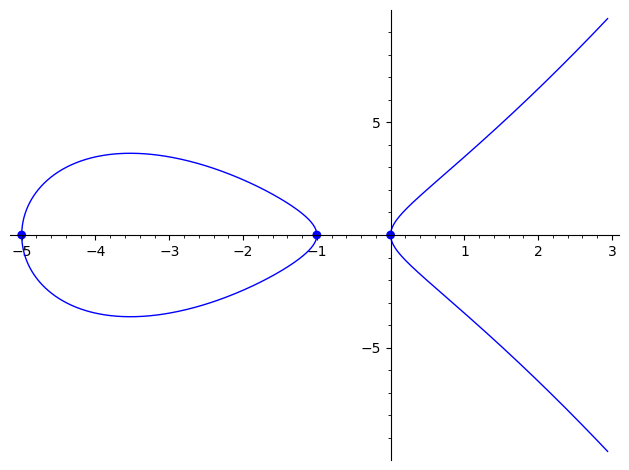
\includegraphics[width=0.3\linewidth]{pointsOfFiniteOrder/examplePointsOfOrder2.png}
    \caption{Points of order 2 on $y^2 = x^3+6x^2 + 5x$ over $\mathbb{Q}$ }%
    \label{fig:pointsOfFiniteOrder/examplePointsOfOrder2}
  \end{figure}
  \noindent
  There are three such points, so we have
  \[ E(\mathbb{Q})[2] = \left\{ \mathcal{O}, (-5 , 0), (-1 , 0 ), (0 , 0) \right\}. \]
  In particular this tells us $E(\mathbb{Q})[2] \simeq \mathbb{Z}/2\mathbb{Z} \times \mathbb{Z}/2\mathbb{Z}$,
  since this is a group of 4 elements and
  all points besides the identity have order 2.
\end{example}
\subsection{The Nagell-Lutz Theorem}%
\label{sub:the_nagell_lutz_theorem}
\begin{theorem} \label{thm:nagellLutz}
  Let $E: y^2 = f(x)$ be an Elliptic Curve over $\mathbb{Q}$.
  All torsion points of $E(\mathbb{Q})$ have integer coordinates.
  Moreover if $(x,y) \in E(\mathbb{Q})_{\tors}$
  and $y = 0$ then $P$ has order 2, else $y|D$,
  the discriminant of $f$.
\end{theorem}

\subsection{Points of Order 2}%
\label{sub:points_of_order_2}

\subsection{Points of Order 3}%
\label{sub:points_of_order_3}
A point $P$ having order $3$ may be phrased as $2P = -P$,
so this means that the $x$ coordinates of $-P$ and $2P$ must be the same.
For an elliptic curve $y^2 = x^3 + ax^2 + bx + c$
one can find that the $x$ coordinate of $2P$ is given by
\begin{equation} \label{eq:xcord2p}
  F(x) = \frac{x^4 -2bx^2 - 8xcx + b^2 - 4ac}{4x^3+4ax^2 + 4bx+4c}
\end{equation}
so a point of order 3 is a fixed point $F(x) = x$, so
\begin{align*}
  F(x) = x &\iff \frac{x^4 -2bx^2 -8cx + b^2 - 4ac}{4x^3+4ax^2 + 4bx+4c} = x \\
           &\iff x^4 -2bx^2 -8xcx + b^2 - 4ac = 4x^4+4ax^3 + 4bx^2+4cx \\
           &\iff \underbrace{3x^{4} + 4ax^3 + 6bx^2 + 12 cx + 4ac - b^2}_{\psi_3} = 0.
\end{align*}
Silverman notes that $\psi_3 = 2f(x)f''(x) - f'(x)^2$ \cite[section 2.1]{silvermanRationalPoints}.
So points of order 3 are roots of this polynomial.
\begin{theorem}
  Let $E: y^2 = f(x)$ be an Elliptic Curve.
  Then $\mathcal{O} \neq P \in E(\mathbb{Q})$ has order 3
  if and only if it is a point of infliction.
\end{theorem}
This result is an exercise in the book of Tate and Silverman
\cite[Exercise 2.2]{silvermanRationalPoints}.
\begin{proof}
  We first find the second derivative, using the chain rule
  \begin{align*}
    \frac{\mathrm{d}^2y}{\mathrm{d}x^2} = \frac{\mathrm{d}^2 \sqrt{y^2} }{\mathrm{d}^2 x}
    = \frac{\mathrm{d}}{\mathrm{d}x} \left[ \frac{\mathrm{d}^2 \sqrt{y^2} }{\mathrm{d}y^2} \frac{\mathrm{d}y^2}{\mathrm{d}x}   \right]
    = \frac{\mathrm{d}}{\mathrm{d}x} \left[ \frac{1}{2 \sqrt{y^2}} f'(x)   \right]
    = \left[\frac{\mathrm{d}}{\mathrm{d}x}\frac{1}{2y} \right] f'(x)
    + \frac{1}{2y} f''(x).
  \end{align*}
  Note that
  \begin{align*}
    \frac{\mathrm{d}}{\mathrm{d}x} \frac{1}{2y} = \frac{\mathrm{d}}{\mathrm{d}y^2} \frac{1}{2y} \frac{\mathrm{d}y^2}{\mathrm{d}x}
    = -\frac{1}{4 y^3} f'(x)
  \end{align*}
  putting this all together we obtain
  \begin{align*}
    \frac{\mathrm{d}^2y}{\mathrm{d}x^2} = -\frac{1}{4y^3} f'(x)^2 + \frac{1}{2y} f''(x)
    = \frac{2y^2}{4y^3} f''(x) - \frac{1}{4y^3}f'(x)^2
    = \frac{2f(x)f''(x) - f'(x)^2}{4yf(x)}
    = \frac{\psi_3(x)}{4y f(x)},
  \end{align*}
  since $y^2 = f(x)$.
  Since a point $(x_0, y_0)$ of order 3 has $\psi_3(x_0) = 0$,
  it follows that $(x_0, y_0)$ is an infliction point
  if and only if $(x_0, y_0)$ has order 3.
\end{proof}
So finding a point of order 3 reduces to finding the roots
of the quartic polynomial $\psi_3$.
From the fundamental theorem of algebra, it then follows
that for every elliptic curve there is a point of order
3 in $E(\mathbb{C})$, but we are interested in rational
points. We shall prove several lemmas which lead up to a
result about points of order 3.
\begin{lemma}
  $\psi_3$ has distinct roots in $\mathbb{C}$.
\end{lemma}
This similar to a result in the book by Tate and Silverman \cite[theorem 2.1]{silvermanRationalPoints}
\begin{proof}
  Recall $\psi_3(x) = 2 f(x)f''(x) - f'(x)^2$, so via the product
  rule
  \[ \psi_3' = 2 \left[ f'f'' + f'''f \right] - 2f'f'' \]
  but $f$ is monic of order 3, so $f''' = 6$, so
  $\psi_3' = 12f$. Since $f$ cannot share any roots with $f'$
  it follows that $\psi_3$ and $\psi_3'$ do not share any roots.
  In conclusion, $\psi_3$ has distinct complex roots.
\end{proof}
\begin{lemma}
  $\psi_3$ has precisely 2 real roots.
\end{lemma}
This is again an exercise in Tate-Silverman \cite[Exercise 2.2b]{silvermanRationalPoints}.
\begin{proof}
  We compute $f''(x) = 6x + 2a$, this has a root $x = -a/3$.
  Since $f'(x) = 3x^2 + 2ax + b$ we find $f'(-a/3) = -a^2/3 -2a^2/3 + b = b - a^2$.
  So
  \[ \psi_3(-a/3) = -(b-a^2)^2 < 0. \]
  But surely the term $3x^4$ is going to be much larger than the lower
  order terms, so at some point $0 \neq x_0 > -a/3$ it is the case that $\psi_3(x_0) > 0$ and $\psi_3(-x_0) > 0$ .
  So by the intermediate value theorem \cite[theorem 4.35]{sutherlandMTS}
  we get the existence of two real roots.

  The coefficients of $\psi_3$ are all real, so we cannot have
  precisely 3 real roots, as then we could find $x_4 \notin \mathbb{R}$
  and so
  \[ \psi_3 = \prod_{i=1}^{4} (x - x_i) = x \prod_{i=1}^{3}(x-x_i) - x_4 \prod_{i=1}^{3} (x - x_i) \notin \mathbb{R}[x].  \]
  So we can only have 2 or 4 real roots.

  Suppose we have $x_1 < x_2 < x_3 < x_4$ real roots, where
  $x_1$ and $x_4$ are the roots we proved exist.
  Then at two points between $x_1$ and $x_4$: $\psi_3' = 12f$ must change sign.
  It follows $f''(x_2) > -a/3$. By the same argument applied to $x_3$ and
  $x_4$ we find $x_3 < -a/3$ so $x_2 > x_3$ which contradicts our ordering.
  Rearranging this argument for all possible orderings of the roots
  can be done similarly.
\end{proof}

\begin{example}
  When $a = 0$ and $c = 0$
  we get an elliptic curve $y^2 = x^3 + bx$
  our $\psi_3$ can be factored easily, since then
  the famous quadratic formula can be used to find
  \begin{align*}
    3x^4 + 6bx^2 - b^2 = 0 &\iff
    x^2 = -b \pm 2/3 \sqrt{3} b
    \iff
    x = \pm \sqrt{-b \pm 2/3 \sqrt{3} b}
  \end{align*}
  so such an elliptic curve never has
  a rational point of order 3 because this $x$ is never rational unless
  $b = 0$, which is a singular curve and hence not elliptic.
\end{example}
\begin{example}
  Consider the curve $E: y^2 = x^3 + x^2 + 2x + 1$ over $\mathbb{Q}$.
  This gives polynomial
  \begin{align*}
    \psi_3 = 3x^4 + 4x^3 + 12x^2 + 12x
  \end{align*}
  which has a rational root $x = 0$.
  Hence the points $(0, \pm 1)$ are of order 3, and moreover these
  are the only points of order 3. Giving us $E(\mathbb{Q})[3] \simeq \mathbb{Z}/3\mathbb{Z}$.
  \begin{figure}[H]
    \centering
    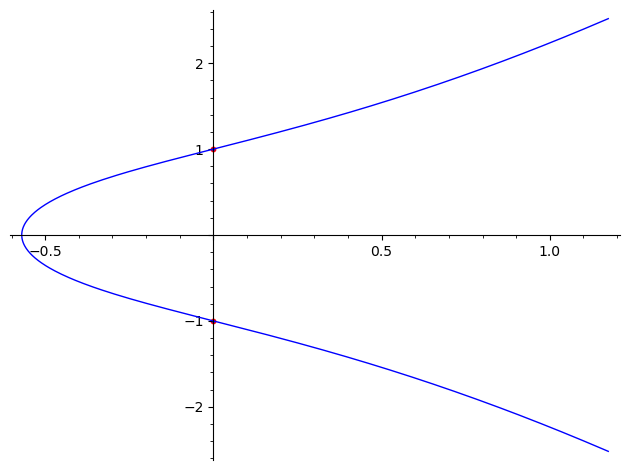
\includegraphics[width=0.4\linewidth]{pointsOfFiniteOrder/examplePointsOrder3.png}
    \caption{Points of order 3 on $y^2 = x^3 + x^2 + 2x + 1$ }%
    \label{fig:pointsOfFiniteOrder/examplePointsOrder3}
  \end{figure}
\end{example}
For some more general Elliptic Curves we can find if a point of order 3 exists as follows.
\begin{corollary}
  Suppose the coefficients of our Elliptic Curve are integers: $a, b, c \in \mathbb{Z}$.
  Then any point of order 3 has $x$-coordinate dividing $4ac - b^2$.
\end{corollary}
\begin{proof}
  From the rational root theorem \cite[Section 9.4]{dummiteAndFooteAbstractAlgebra}
  any rational root of $\psi_3$ has the form $x = p/q$ where $\gcd(p, q) = 1$, $p | 4ac - b^2$ and $q|3$,
  moreover we know from theorem \ref{thm:nagellLutz}
  that $p/q \in \mathbb{Z}$, so $q | p$. If $q = 3$ then $\gcd(p, q) = 3$
  which is not in lowest terms, so we have $q = 1$.
  For any rational solution $x$ we have $x|4ac - b^2$.
\end{proof}
\begin{example}
  For the Elliptic Curve
  $y^2 = x^3 + 3x^2 + 3x + 2$ we have
  any rational solution $x$ has
  $x|15$.
  By trying all divisors of $15$ we find $\psi_3(-1) = 0$ and
  hence we conclude $(0,-1)$ is a point of order 3.
\end{example}
\begin{example}
  The Elliptic Curve $y^2 = x^3 -9x + 9$
  has $b^2 - 4ac = -81$, which has divisors
  $\pm 1, \pm 3, \pm 9, \pm 81$.
  So by trial and error on
  \begin{align*}
    \psi_3 = 3x^4 - 54x^2 + 108x - 81
  \end{align*}
  we find that $\psi(3) = 0$.
  Hence $(3, \pm 3)$ are points of order 3.
\end{example}
\begin{example}
  The curve $y^2 = x^3 + 1$ is quite interesting.
  Since it contains both a point of order 2 and a point of order 3,
  clearly $-1$ is a root of $x^3 + 1$, which corresponds to a point (0, -1) of order 2,
  while $0$ is a root of $\psi_3$ so $(\pm 1, 0)$ are points of order 3.
  So we multiply a point of order 2 with a point of order 3 to give us a point of order 6,
  namely the point $(3, 2)$ has order 6.
\end{example}
